%%
%% Edward T. Norris
%% Discrete Ordinates Computed Tomography Organ Dose Simulator (DOCTORS)
%% 
%% === Implementation ===
%%

This chapter covers the details of the implementation of the different components of the DOCTORS code base. The code is available from a GitHub Git repository. At the time of this writing, the repository is located at \texttt{https://github.com/eNorris/thesis} and is only available subject to special request and license agreement. An executable version can also be made available upon request. An executable-only public release is planned for the future.

The code is implemented in C++ and requires a C0x11 compliant compiler. The user interface is written using the Qt5 framework. GPU computation is performed via CUDA which must be compiled seperatly by Nvidia's proprietary compiler, \texttt{nvcc}.

Unless noted otherwise, all code listings are formatted as C++ code though some parts of the code may be omitted. Omissions include typical "boiler plate" code that accompanies all code such as the \texttt{\#include} statements and any \texttt{using namespace} commands. Additionally, the \texttt{main()} function and others are omitted, showing only the code relevant to the discussion.

\section{Vector Flattening}\label{sec:flatten}

Data is stored in large, multi-dimensional arrays. For example, the CT voxel phantom can be intuitively stored as a 3D array of floating precision values which can be easily indexed. However, DOCTORS is written such that it is extensible to GPUs. GPUs are not optimized for data stored in a multi-dimensional fashion, but rather for data stored as a single 1-dimensional array. To emulate the 3-dimensional storage arrangement of the data, indexing arithmetic is used.

On the CPU, data is stored as C++ \texttt{std::vector<T>} objects where the \texttt{T} template parameter can be either \texttt{float} or \texttt{double} depending on the precision (32 bits or 64 bits respectively) needed. The storage space available to a \texttt{std::vector<T>} object is effectively unlimited, bounded only by the host CPU's physical RAM. However, other effects such as memory fragmentation can limit the practical size of a single, continuous \texttt{std::vector<T>} object significantly. To emulate indexing of a $N_x \times N_y$ matrix, a single \texttt{std::vector<T>} is created and resized to $N_x \times N_y$ elements. The global index, $i$, in the flattened array is then
\begin{equation}
i = i_x N_y + i_y.
\end{equation}
This pattern extends to multi-dimensional matrices. For example, a $N_x \times N_y \times N_z$ matrix would be globally indexed as
\begin{equation}
i = i_x N_y N_z + i_y N_z + i_z.
\end{equation}

Figure~\ref{fig:indx_ex} gives an example of the spatial indexing scheme using an $8 \times 8 \times 8$ mesh. The indicated voxel has $i_x$, $i_y$, and $i_z$ indices of 1, 5, and 6 respectively. Therefore, the index value of the highlighted voxel is $1 \times 8 \times 8 + 5 \times 8 + 6$ = 110. This flattening pattern continues to higher dimensional phase space to encompas energy and direction.

\begin{figure}[tb]
  \begin{center}
   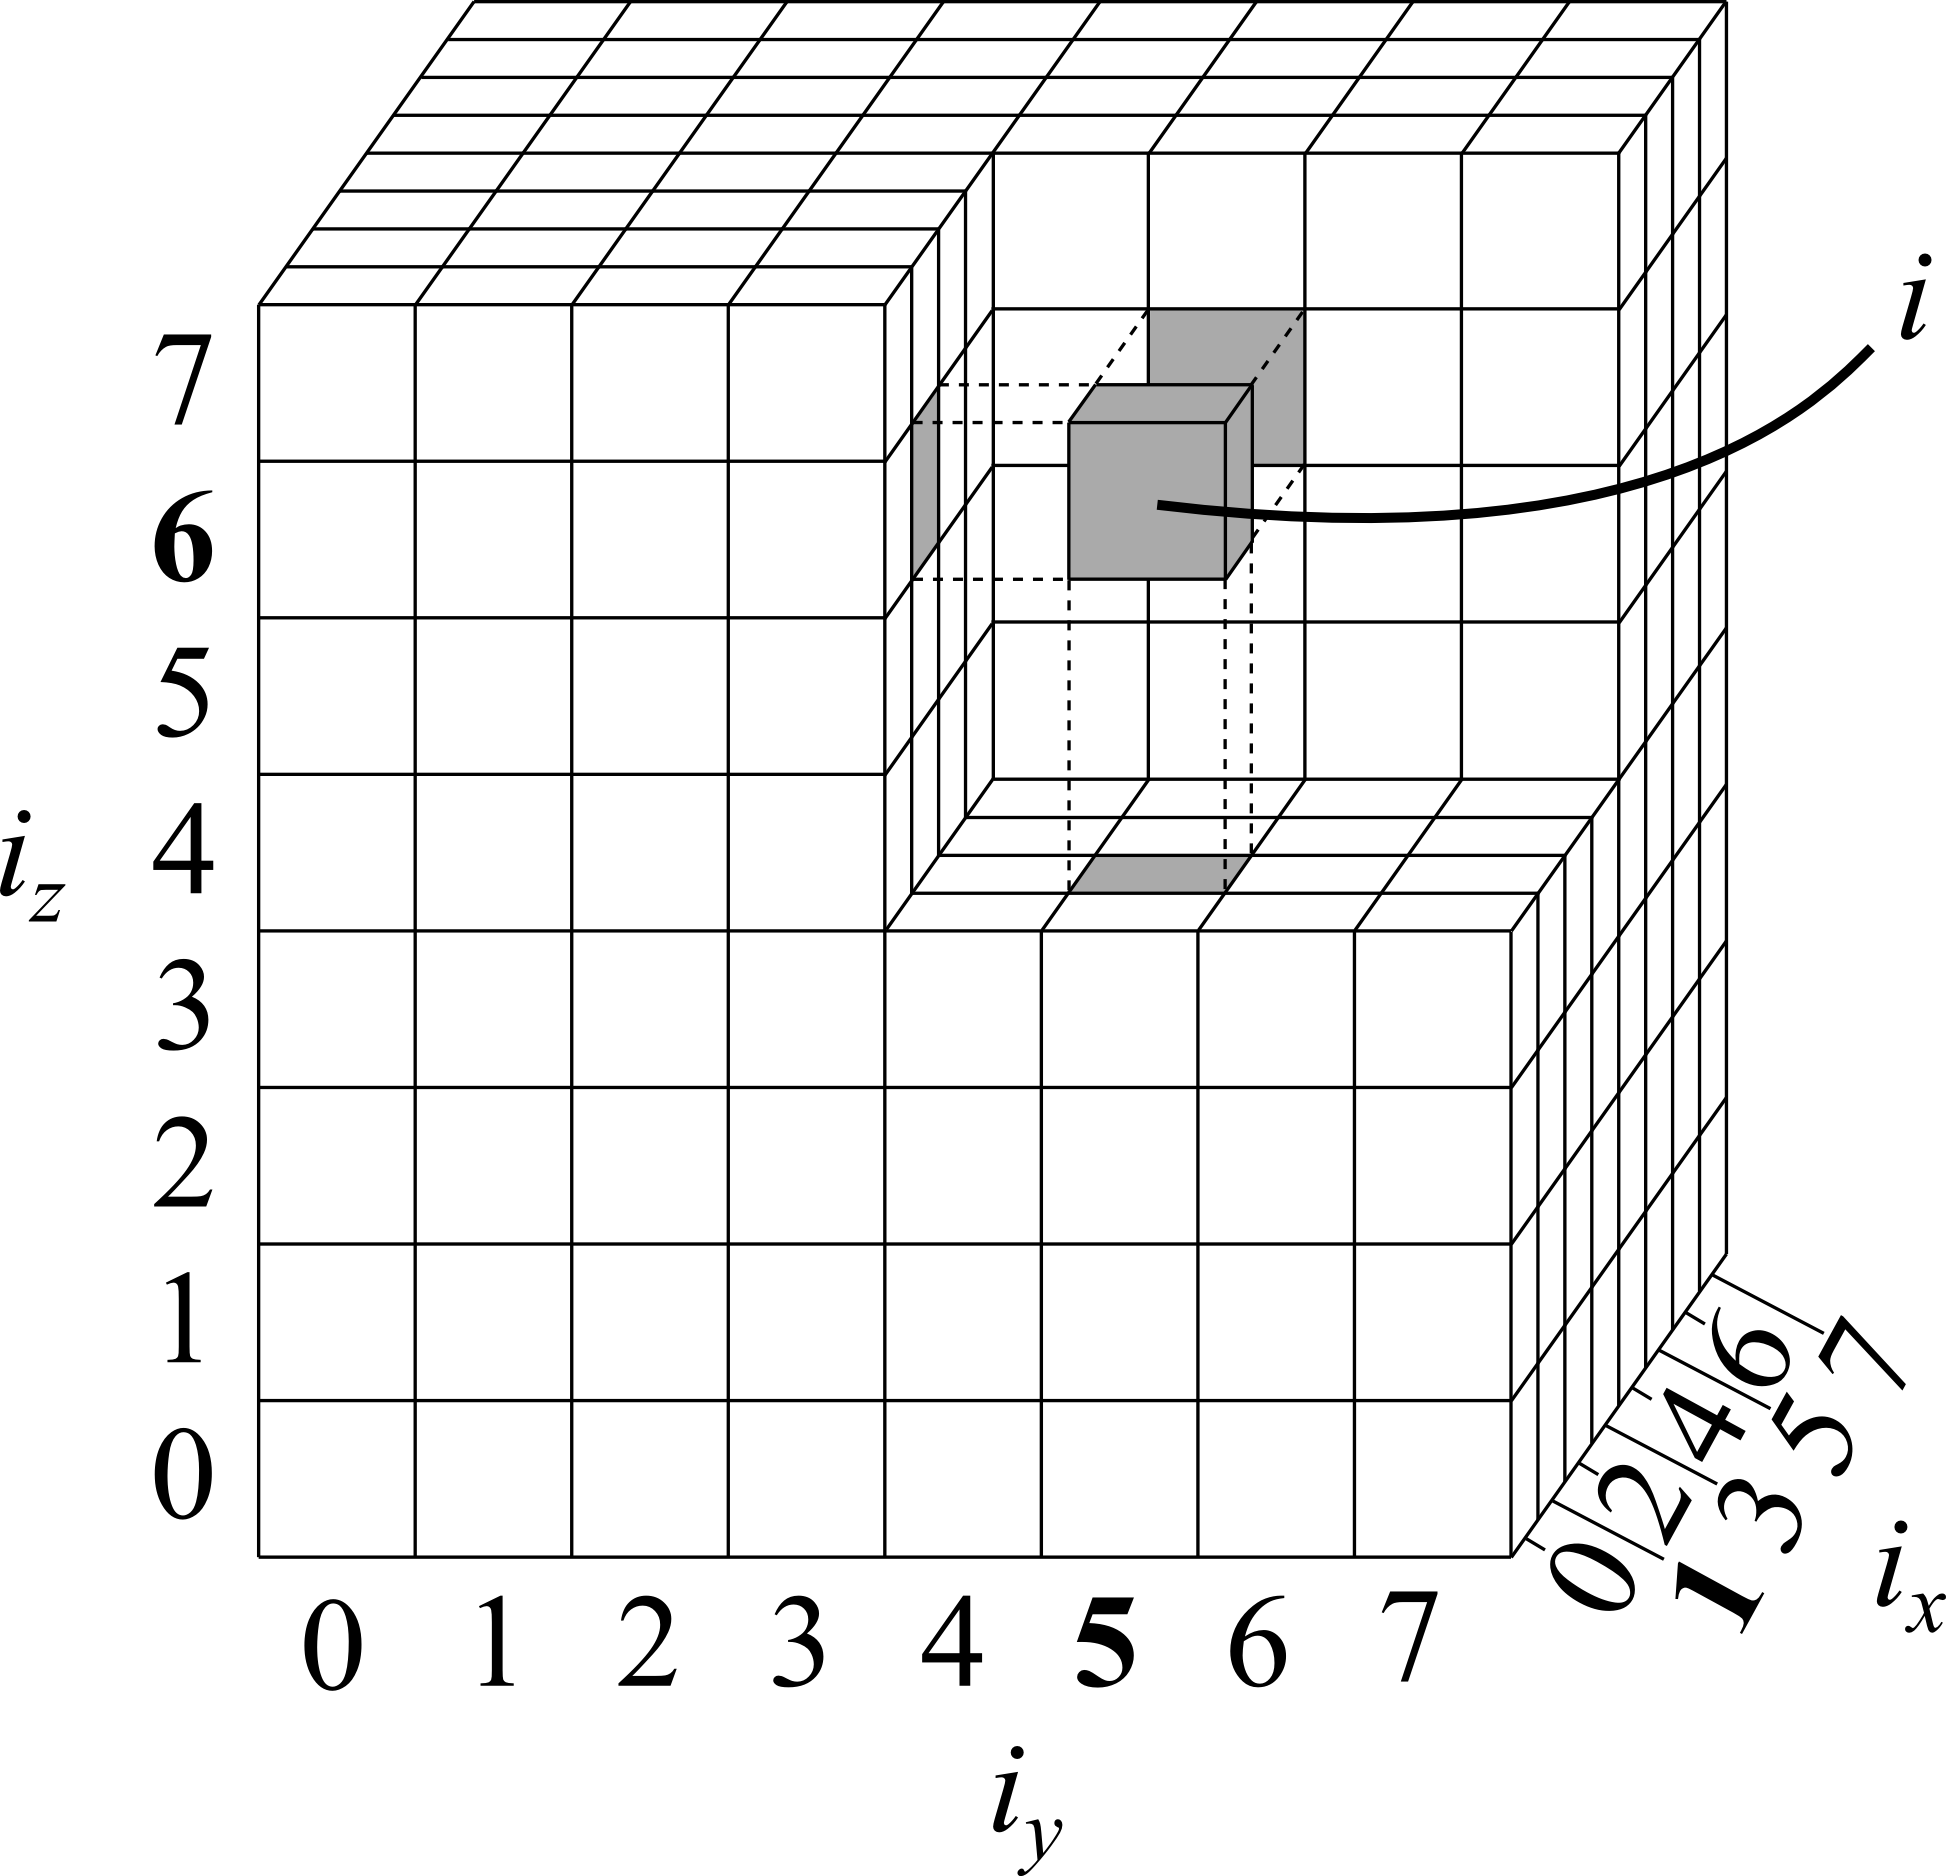
\includegraphics[width=3.75in]{figs/indx_ex}
  \end{center}
  \caption{Conversion from 3D indexing to 1D "flattened" indexing.}
\label{fig:indx_ex}
\end{figure}

A variable that is dependent on $x$, $y$, $z$, $E$, and $\Omega$ would be written as $\phi(x, y, z, E, \Omega)$ would be discretized to $\phi(i_x, i_y, i_z, G, i_a)$. Rather than storing $\phi$ as a 5-dimensional matrix, $\phi$ is stored as a 1-dimensional vector of the same number of elements.

\section{Cross Section Parsing}\label{sec:xsparse}
AMPX cross sections are stored in a binary format. These files are \textit{not} distributed with DOCTORS but must be obtained from SCALE6.2 or another code. Figure~\ref{fig:ampx} shows the data format of the overall file. The binary file is split into a sequence of records. The header section of the file has overall information about the file including the number of nuclides stored, their energy group structure, and a comment string describing the file. Following the header section is a list of directory records. Each directory has information about a specific nuclide including the cross section reaction types available, temperatures for which the cross sections were evaluated, the number of Legendre expansion coefficients stored in the scatter matrix, and other data. Following the directories, more records follow that describe the energy structure used in the file. There is one such record for each particle type. The libraries used in the current version of DOCTORS have both neutron and photon cross section data stored.

The file header section, directories, and energy group boundaries describe the structural information necessary to read the following nuclide records. Nuclides are listed in the same order their directories are found after the header setion. Each nuclide contains numerous records.

\begin{figure}
    \centering
    \begin{subfigure}[b]{0.45\textwidth}
        \includegraphics[width=\textwidth]{figs/ampx1}
        \caption{}
        \label{fig:ampx1}
    \end{subfigure}
    ~
    \begin{subfigure}[b]{0.45\textwidth}
        \includegraphics[width=\textwidth]{figs/ampx2}
        \caption{}
        \label{fig:ampx2}
    \end{subfigure}
    \caption{The format of the AMPX file. (a) The file contains a header, a list of directory records, energy group information and a list of nuclide entries. (b) Each nuclide entry contains multiple records; the two of concern in this work are the last two containing gamma data.}\label{fig:ampx}
\end{figure}

Each record contains a string of data bytes between a four byte header and four byte footer. The header and footer are identical and, when interpreted as a signed four byte integer, give the size in bytes of the record. An example record is shown in Fig.~\ref{fig:ampxbytes1}.

The data is stored in Big Endian format which must be converted to Little Endian for most Intel and AMD processors.  The endianess rearrangement is shown in Fig.~\ref{fig:ampxbytes2}. Each record is one of 12 unique types; each type of record is formatted and interpreted differently. For example, Type 1 contains general information about the data file such as the number of nuclides, number of energy groups, and a brief description. Type 2 records contains a list of floating-point numbers representing the energy group boundaries. Figure~\ref{fig:ampxbytes1} shows a Type 1 record. In the case of the header bytes given in Fig.~\ref{fig:ampxbytes1} and~\ref{fig:ampxbytes2}, the bytes correspond to the integer 440 which is the length in bytes of the record (not including the header or footer). Each byte of data is sequentially read, reordered, and converted to an apprpriately typed variable. Table~\ref{tab:reorder} shows the converstion for the record given in Fig.~\ref{fig:ampxbytes1}.

\begin{figure}[tb]
  \begin{center}
   \includegraphics[width=4.75in]{figs/ampxbytes1}
  \end{center}
  \caption{An example record parsed. The header and footer are identical and equal to the number of bytes in the record.}
\label{fig:ampxbytes1}
\end{figure}

\begin{figure}[tb]
  \begin{center}
   \includegraphics[width=4.75in]{figs/ampxbytes2}
  \end{center}
  \caption{The byte reordering from Big Endian to Little Endian. Individual bits within a byte are not rearranged, but the ordering of the four bytes withing a 32-bit word is reversed.}
\label{fig:ampxbytes2}
\end{figure}

\begin{table}[ht]
\caption{Byte Reordering}
\centering 
\begin{tabular}{l | c | c | c | l}
  \hline \hline   
  Word  & Big Endian & Little Endian & Interpreted & Notes\\ [0.5ex] % inserts table 
  \hline
  0   & B8 01 00 00 & 00 00 01 B8 & 440    & Header                    \\
  1   & 8B 69 00 00 & 00 00 69 8B & 27019  & ID                        \\
  2   & A4 01 00 00 & 00 00 01 A4 & 420    & Number of nuclides        \\
  ... &      ---    &      ---    &    --- & ---                       \\
  11  & 70 75 6F 43 & 43 6F 75 70 & "Coup" & First four \texttt{char} of the title   \\
  12  & 20 64 65 6C & 6C 65 64 20 & "led " & Second four \texttt{char} of the title  \\
  ... &     ---     &    ---      &  ---   & ---                       \\
  110 & 20 20 20 20 & 20 20 20 20 & "    " & 4 spaces ending the title \\
  111 & B8 01 00 00 & 00 00 01 B8 & 440    & Footer                    \\ 
  [1ex]      % [1ex] adds vertical space
  \hline
\end{tabular}
\label{tab:reorder}
\end{table}

The header always reports the number of 8-bit bytes required to store the data. However, some data types, such as \texttt{char}, are only one byte so each word represents multiple (4 in the case of \texttt{char}) distinct characters.


The first entry in each nuclide entry is the directory record. The directory contains general information regarding the nuclide and information necessary to parse the proceeding records. Following the directory, Bondarenko data, resonance parameters, neutron data, and gamma production which are not of interest in photon only problems are read.

The penultimate record contains the average cross section data. This data is averaged over all energies and directions using Eq.~\ref{eq:groupxs}. The only data used in this section in DOCTORS is the total cross section values necessary for implementing the fully discretized form of the LBE given in Eq.~\ref{eq:boltz_i}.

The 2D data is stored in a special format optimized for scatter matrix data. The format concists of a sequence of "magic numbers" interpersed within a list of data points. A magic number is a nine digit number IIIJJJKKK. The first three digits, III, are the group number of the highest energy group to scatter to the energy of interest. The next three digits, JJJ, are the group number of the lowest energy to scatter. The final three digits, KKK, are the group number of the sink energy to which particles are scattering. Given a magic number \texttt{magic}, the three values can be computed in Listing~\ref{lst:magic}. Note that the group numbers are indexed from 1 to $G$ instead of 0 to $G-1$ as required by DOCTORS. This is corrected by subtracting 1 while doing the indexing arithmetic.

\begin{listing}
\begin{minted}[frame=lines,linenos]{c++}
magic = READ_NEXT_BINARY_INT()
KKK = magic % 1000
JJJ = (magic % 1000000 - KKK) /1000
III = (magic - JJJ - KKK) / 1000000

src = JJJ
while src >= III
	data = READ_NEXT_BINARY_FLOAT()
	xs[(src - 1)*G + KKK - 1] = data
	src = src - 1
\end{minted}
\caption{Computation of the source and sink groups from the magic number and the subsequent data parsing.}\label{lst:magic}
\end{listing}

Figure~\ref{fig:sigmacomp} shows the microscopic cross section data pulled from the 200-neutron/47-gamma group data file currently used by DOCTORS for hydrogen and oxygen. The data is compared to reference data pulled directly from the ENDF/B-VII.1 photoatomic (MT=501) data library~\citep{ref:cullend} accessible through the Sigma database~\citep{ref:sigma}.

\begin{figure}
    \centering
    \begin{subfigure}[b]{0.45\textwidth}
        \includegraphics[width=\textwidth]{figs/sigmacomp1}
        \caption{}
        \label{fig:ampx1}
    \end{subfigure}
    ~
    \begin{subfigure}[b]{0.45\textwidth}
        \includegraphics[width=\textwidth]{figs/sigmacomp2}
        \caption{}
        \label{fig:ampx2}
    \end{subfigure}
    \caption{The microscopic cross section in bars for hydrogen and oxygen. Both subfigures show identical data, (a) shows the entire data range available in the reference data library and (b) shows only the data range applicable to DOCTORS.}\label{fig:sigmacomp}
\end{figure}

\section{Generation of Material Cross Section Data}\label{sec:xsgen}

Once the data is parsed, weighted combinations of elemental data is used to create material cross sections. Cross section data for photons always uses the naturally ocurring since photo-atomic reactions are not sensitive to the nuclear differences between isotopes. The compositions of N materials are assumed to be given as weight fractions, $w_i$ subject to
\begin{equation}
\sum_{i = 1}^N w_i = 1
\end{equation}
and is converted to an atom fraction, $a_i$:
\begin{equation}
a_i = \frac{w_i}{M m_i}
\end{equation}
where
\begin{equation}
M = \sum_{i = 1}^N \frac{w_i}{m_i}
\end{equation}
and $m_i$ is the element's atomic weight.

In the solution employed by DOCTORS, only the total and scattering cross sections are required. The AMPX data files however, support arbitrary reaction types and have up to a dozen or more reactions for photo-atomic reactions alone for elemental datasets. The reaction types are identified by their MT designation. The total, inelastic, and elastic scatter cross sections are MT 501, 502, and 504 respectively. The scatter cross section used by DOCTORS is the sum of the elastic and inelastic cross sections.

The cross section of compound materials are computed as a weighted summation of their components. For example, the cross section of water for a particular reaction would be
\begin{equation}
\sigma_{H_2 O} = \frac{2 \sigma_H + \sigma_O}{3}.
\end{equation}

\begin{figure}
    \centering
    \begin{subfigure}[b]{0.45\textwidth}
        \includegraphics[width=\textwidth]{figs/airwaterxs2_19group}
        \caption{19 group data}
        \label{fig:airwaterxs2_19group}
    \end{subfigure}
    ~
    \begin{subfigure}[b]{0.45\textwidth}
        \includegraphics[width=\textwidth]{figs/airwaterxs2_47group}
        \caption{47 group data.}
        \label{fig:airwaterxs2_47group}
    \end{subfigure}
    \caption{Comparison of the group-averaged DOCTORS cross section data to continuous NIST data.}\label{fig:airwaterxs_group}
\end{figure}

\section{Qt5 Framework}\label{sec:qt}
The Qt5 framework was used for implementation of the user interface. Qt5 enables asynchronous calls through its signal/slot mechanism. Signals and slots are special functions that have additional processing performed by the meta-object-compiler (MOC). A signal can be emitted which will execute all connected slots. Signals and slots are connected manually by the user except special ones automatically generated by Qt5. 

Qt5 prvides a user interface for building user interfaces. Components such as buttons, drop boxes, radio buttons, etc. are made available to the user. Through extensive use of polymorphism, Qt5 simplifies the addition of graphical interactive elements called widgets. All widgets inherit from the base \texttt{QWidget} class which inherits from \texttt{QObject}. Any class that utilizes the signal/slot mechanism must extend the \texttt{QOjbect} class. As an example, a button can be created in the Qt5 user interface and named \texttt{button1}. This object will be accessible as \texttt{ui->button1}. When the user clicks on the button, the signal \texttt{button1.clicked()} will automatically be emitted. The user can connect this signal to any slot with an identical number arguments of the same type. The \texttt{button1.clicked()} signal can be connected to the slot \texttt{doStuff1()} but not \texttt{doStuff2(int)} since the arguments are not compatible.

Listing~\ref{lst:sync1} gives a C++ snippet that has a long function that will block the user interface. A corresponding sequence diagram is given in Fig.~\ref{fig:sync1}. When the user interacts with the GUI, the writer object begins executing the \texttt{doWrite()} function. Until this function completes, the UI thread will be busy and unable to handle additional user interaction or updates. This results in the GUI becoming unresponsive and potentially issuing a warning to the user from the operating system. The code in Listing~\ref{lst:sync1} is updated to use the Qt signal/slot mechanism whose code is given in Listing~\ref{lst:async1}.

\begin{listing}
\begin{minted}[frame=lines,linenos]{c++}
class MainWindow : public QMainWindow
{
	// Constructor
	MainWindow(QObject *parent);
	
	// Other parts of the class
	
protected slots:
	void doSomethingLong();
}

void MainWindow::doSomethingLong()
{
	// Execute a long piece of code
}
	

MainWindow::MainWindow(QObject *parent)
{
	// Initializations
	
	// When a button named button1 which was created in the Qt5
	//   creator interface is clicked, the clicked() signal is 
	//   automatically emitted which executes the doSomethingLong()
	//   function
	connect(ui->button1, clicked(), this, 
		doSomethingLong());
}
\end{minted}
\caption{A long function causes the user interface to block.}\label{lst:sync1}
\end{listing}

\begin{listing}
\begin{minted}[frame=lines,linenos]{c++}
class MainWindow : public QWindow
{
	// Member variables
	QThread workerThread;
	Worker *worker;
	
	// Constructor
	MainWindow(QObject *parent);
	
protected slots:
	handleResult();
}
	
MainWindow::MainWindow(QObject *parent)
{
	// Initializations
	worker = new Worker;
	
	worker.moveToThread(&workerThread);
	
	// Set up the thread connections
	connect(&workerThread, finished(), worker, deleteLater());
	connect(this, begin(), worker, doSomethingLong());
	connect(worker, done(), this, handleResult());
}

class Worker : public QObject
{
private signals:
	void done();
	
public slots:
	void soSomethingLong();
}

Worker::doSomethingLong()
{
	// Do stuff...
	emit done();
}

\end{minted}
\caption{Signals and slots enable a long function to be called without blocking the user interface.}\label{lst:async1}
\end{listing}

\begin{figure}[tb]
  \begin{center}
   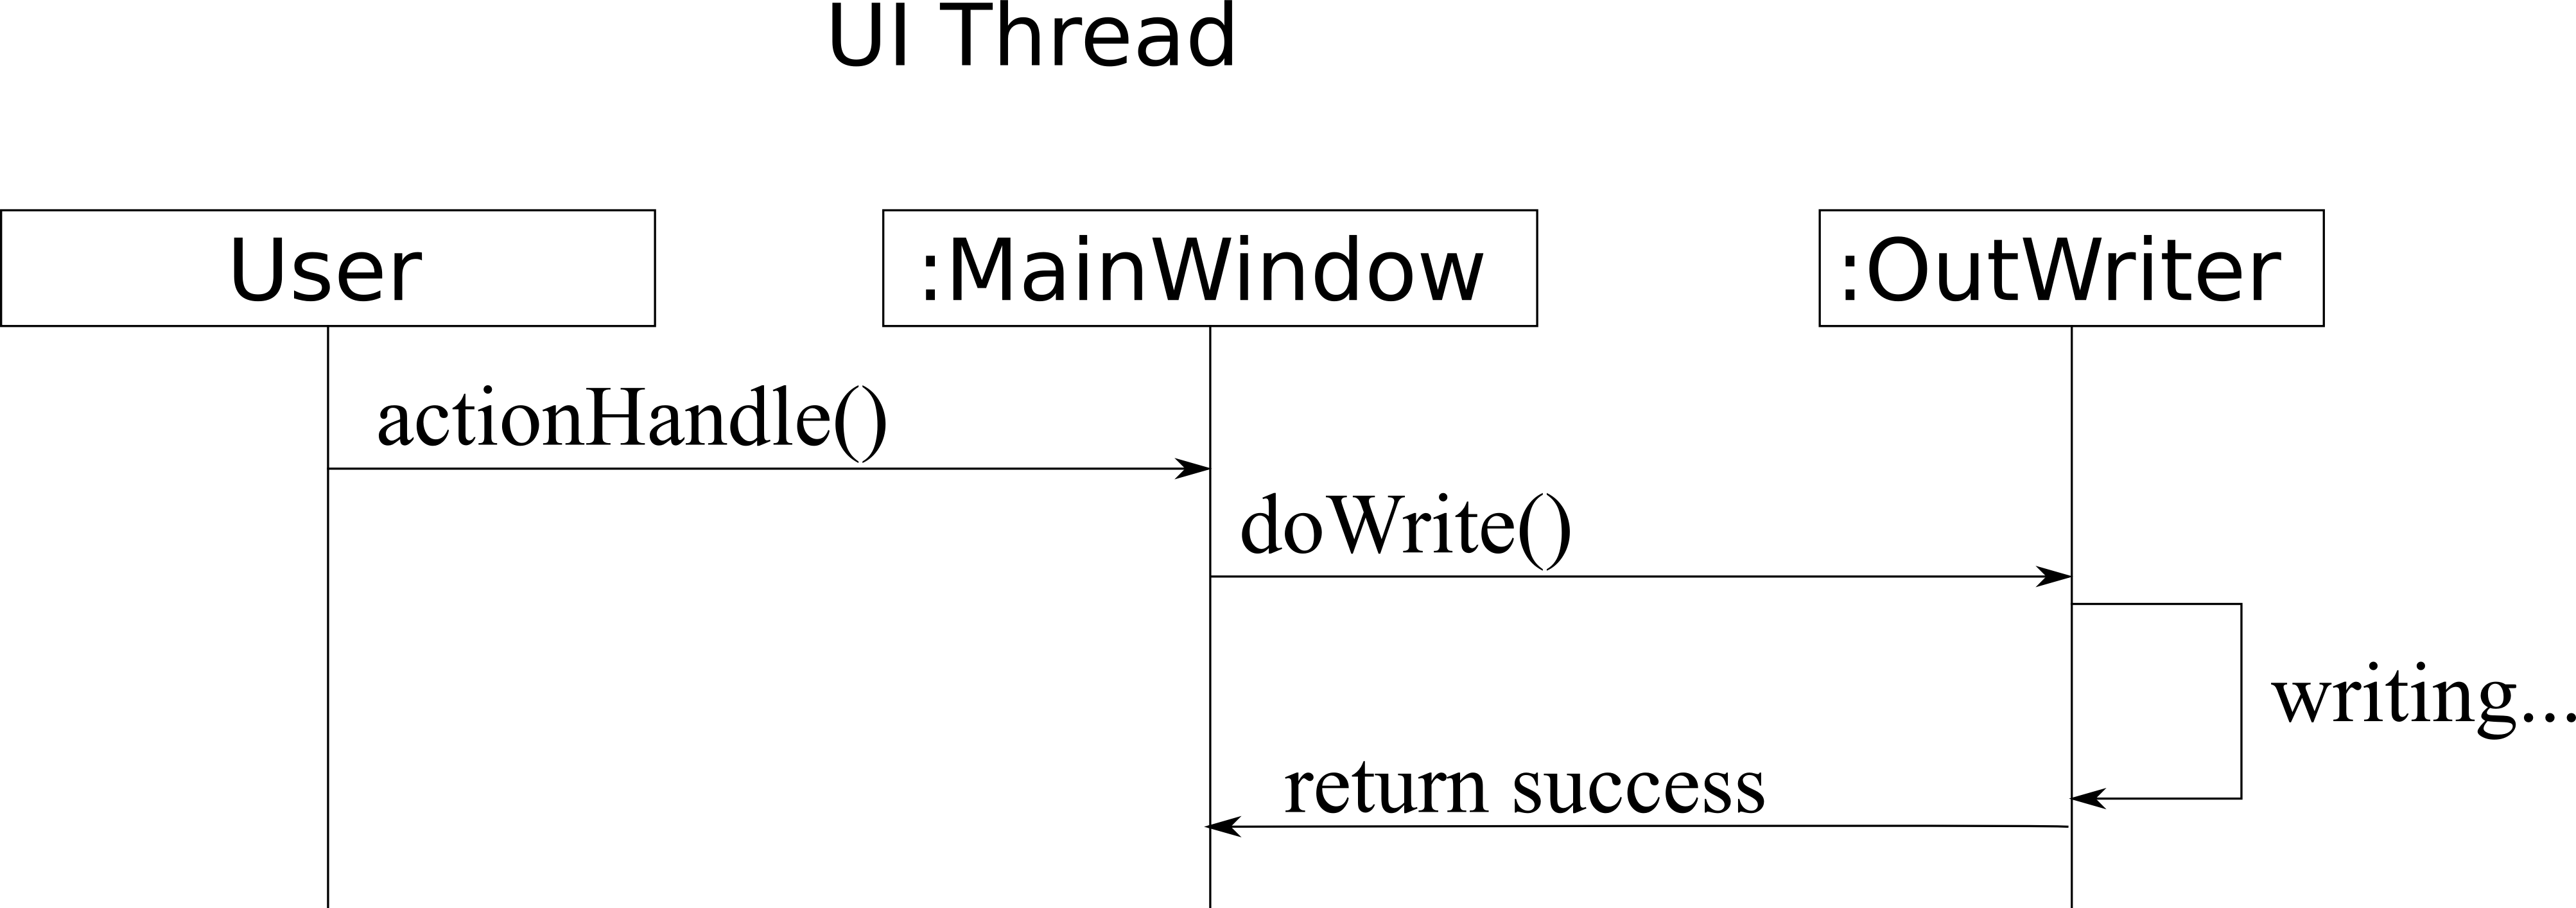
\includegraphics[width=3.75in]{figs/writer_sync}
  \end{center}
  \caption{Sequence diagram for the synchronous call.}
\label{fig:sync1}
\end{figure}

\begin{figure}[tb]
  \begin{center}
   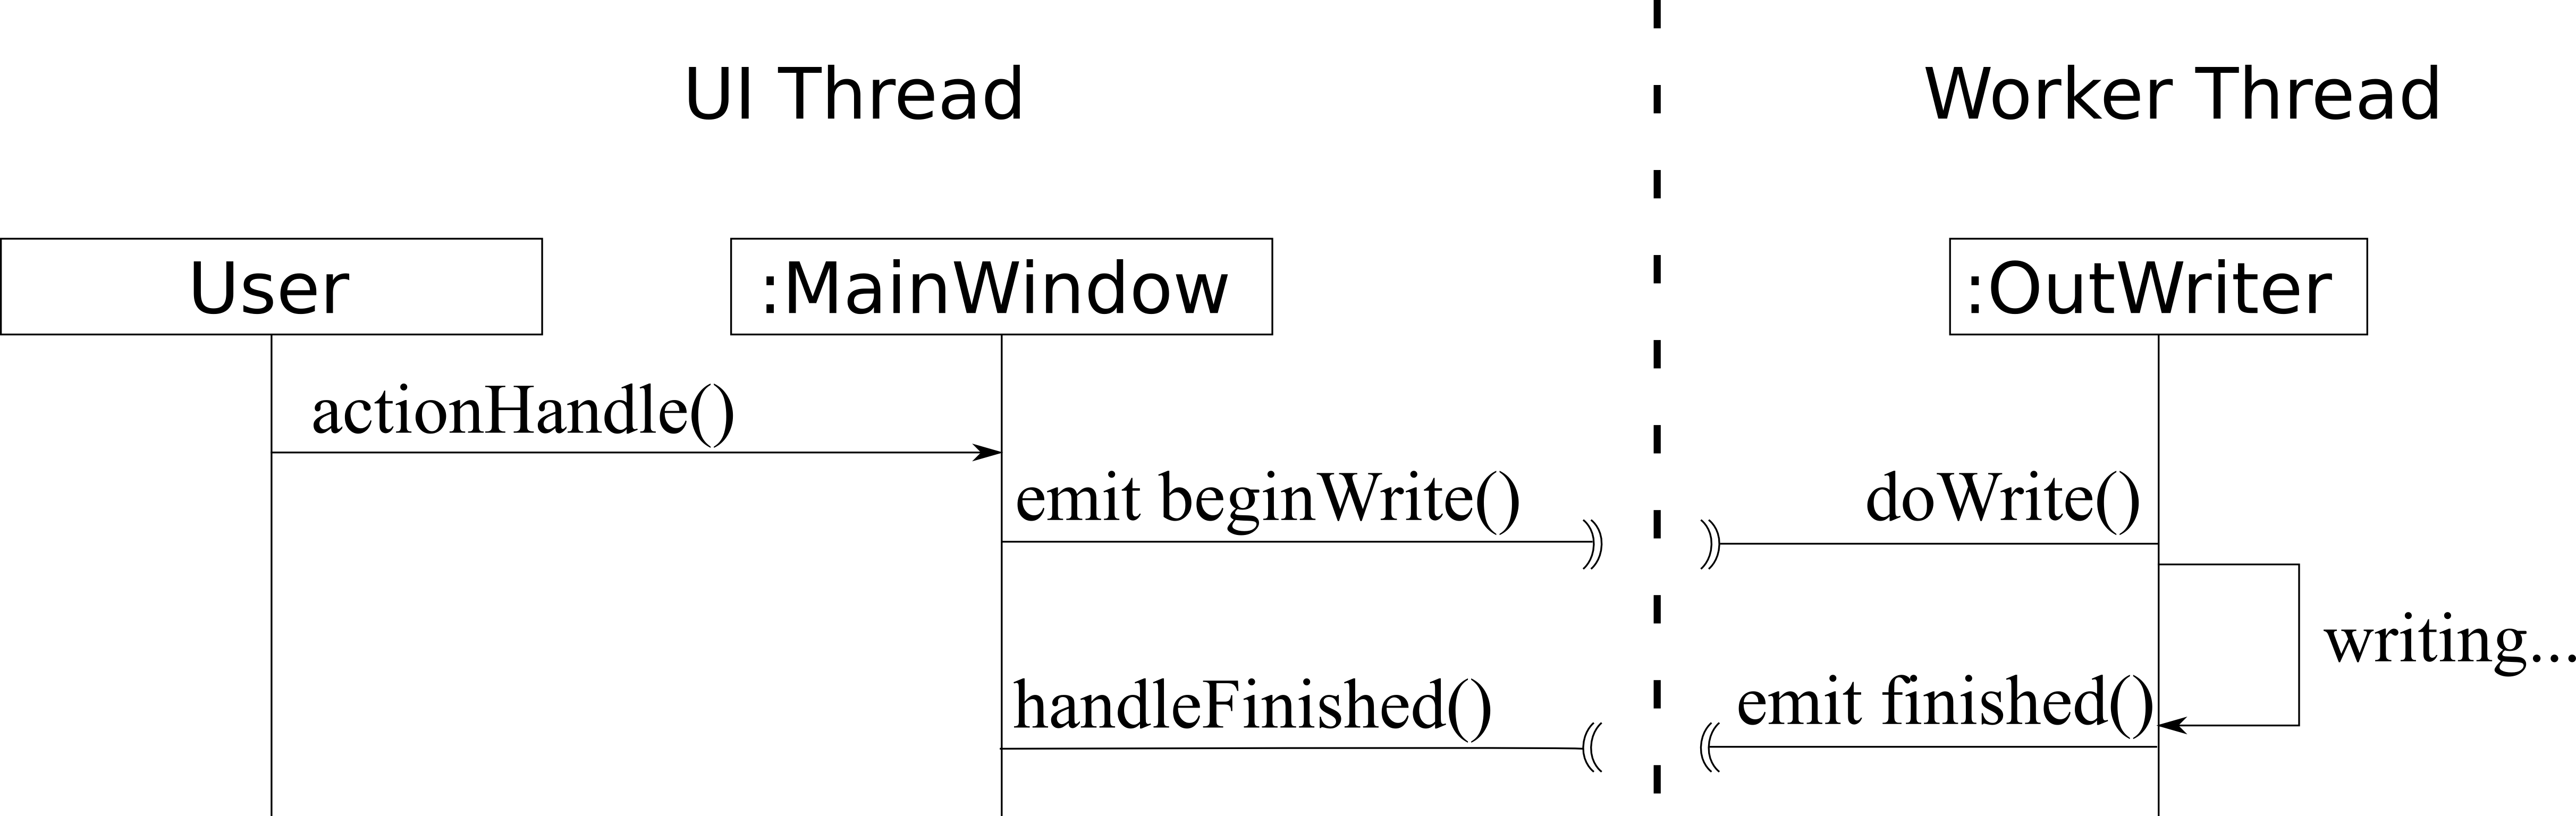
\includegraphics[width=3.75in]{figs/writer_async}
  \end{center}
  \caption{Sequence diagram for the synchronous call.}
\label{fig:async1}
\end{figure}

\section{Graphical User Interface}\label{sec:gui}

The data display plots that show materials and other geometry as well as the flux output use an implementation of the built-in \texttt{QGraphicsView} object to render a matrix of \texttt{QGraphicsRectItem}s on the screen. The data to be drawn on the screen is populated and some metrics such as the dataset minimum and maximum are computed. The data value at each point is evaluated to determine which bin it belongs to. 

The first tab is the geometry input, shown in Fig.~\ref{fig:gui_tab1}. In the current version of DOCTORS, the only supported format is unsigned 16-bit binary files whose size is known \textit{a priori}. When the user clicks on the "Open" button, the user is prompted with a dialog for selection of a binary file. The file is read in as a list of $N_x \times N_y \times N_z$ CT numbers. As soon as the data is read in and some checks are performed, the user is prompted for selection of a CT-number-to-material conversion. Currently, two conversions are included in DOCTORS. The first is a water/air only conversion and the second is a more complex conversion to a series of dosimetrically equivalent materials representative of a human patient. Once the user specifies a conversion, the geometry explorer becomes available which allows the user to visualize the geometry file to verify that it was read and interpreted correctly.

\begin{figure}[tb]
  \begin{center}
   \includegraphics[width=3.75in]{figs/gui3}
  \end{center}
  \caption{The geometry selection tab. The user must first specify the dimensionality of the voxel phantom and then load it from a binary file.}
\label{fig:gui_tab1}
\end{figure}

Some screenshots of the geometry explorer are shown in Fig.~\ref{fig:gui_geom}. The geometry viewer can show slices through the voxel phantom along all three major planes. The depth of the slice viewed is changed by moving the scroll bar in the center of the viewer up or down. As the scroll bar moves, the number at its bottom is updated accordingly to indicate the depth (in voxels) of the slice. In addition to the material, the geometry viewer can render the physical density (in g/cm$^3$) and the atom density (in atom/b-cm) as well as the raw CT number used to generate the material and density.

\begin{figure}
    \centering
    \begin{subfigure}[b]{0.45\textwidth}
        \includegraphics[width=\textwidth]{figs/gui1}
        \caption{}
        \label{fig:gui1}
    \end{subfigure}
    ~
    \begin{subfigure}[b]{0.45\textwidth}
        \includegraphics[width=\textwidth]{figs/gui4}
        \caption{}
        \label{fig:gui4}
    \end{subfigure}
    \caption{The geometry explorer. (a) The material viewer which shows which material each voxel was converted to. (b) The atom density plot.}\label{fig:gui_geom}
\end{figure}

The next three tabs identify the cross section dataset to use for the material generation, the quadrature, and the solution anisotropy treatment used. All three tabs are relatively strightforward and contain few widgets. The final tab, shown in Fig.~\ref{fig:gui_src} defines the source. The user is presented with a number of different source geometries to choose from. Each type is described more fully in Sec.~\ref{sec:source_gen}. Clicking on the "Energy Distribution" button will reveal the popup shown in Fig.~\ref{fig:gui_spect}. This popup cannot be fully populated until \textit{after} the cross section is loaded in the "Cross Section" tab since the cross section data file defines the energy group structure.

The energy distribution dialog, shown in Fig.~\ref{fig:gui_spect}, can plot the $x$ axis on either a linear or logarithmic scale. The user can click and drag to "paint" a spectrum to generate quick, qualitative spectra suiting the user's needs. Alternatively, the user can select from any of the preset spectra in the dropdown menu. Currently, only the uniform beam and diagnostic pulse distributions described later are present.

\begin{figure}[tb]
  \begin{center}
   \includegraphics[width=3.75in]{figs/gui2}
  \end{center}
  \caption{The source tab. The user must select a geometry type and enter all applicable values as well as define the source energy spectrum.}
\label{fig:gui_src}
\end{figure}

\begin{figure}[tb]
  \begin{center}
   \includegraphics[width=3.75in]{figs/gui6}
  \end{center}
  \caption{The spectrum energy distribution. The spectrum can be displayed on either a linear or logarithmic scale on the $x$ axis. The user can either click and drag on the spectrum to "paint" or select a preset.}
\label{fig:gui_spect}
\end{figure}

Once all necessary data is loaded, the "Launch" button becomes active and will remain so until the user creates a conflicting set of input that would prevent the solver from being able to run. When the user clicks on the launch button, the raytracer begins running asynchronously and the output display shown in Fig.~\ref{fig:gui_out} opens automatically. When the raytracer completes, the output dialog is updated with the flux information and the solver begins executing asynchronously. As each iteration completes, the output dialog is progressively updated so that the user can monitor the evolution of the solution.

The output dialog has controls very similar to the geometry explorer. The user can freely choose the plane to slice through the solution and can plot the solution on either a linear or logarithmic scale. The "Distribution" radio buttons allows the user to choose whether the uncollided, collided, or total flux is shown. The "Level Local Scale" checkbox allows the user to control whether the current slice colormap is scaled to the contents of the viewed slice or the contents of the entire voxel phantom. Checking the "Level Local Scale" box will ensure that the viewed data is normalized to include only the viewed data. Unchecking the box will scale the viewed data based on the range of the entire voxel phantom.

\begin{figure}[tb]
  \begin{center}
   \includegraphics[width=3.75in]{figs/gui5}
  \end{center}
  \caption{The output dialog. The controls are similar to those found in the geometry viewer.}
\label{fig:gui_out}
\end{figure}

In the current version of DOCTORS, dosimetric output is only written to an output file and cannot be visualized graphically. The output format is designed to be human readable and easily read by any major programming language. Listing~\ref{lst:output_fmt} gives the code to read the file format where the \texttt{prod()} algorithm is given in Listing~\ref{lst:prod}. Note that \texttt{LIST} may be any appropriately typed list object such as a \texttt{std::vector} and a \texttt{LIST2D} is a list of lists or vector of vectors.

\begin{listing}
\begin{minted}[frame=lines,linenos]{c++}
// Declare variables
int N;
LIST S;
LIST2D dims;
LIST data;

// Read the number of dimensions
READ_INT(N);

// Read the size of each dimension
for(int i = 0; i < N; i++)
	READ_INT(S[i]);
	
// Read the axis labels
for(int i = 0; i < N; i++)
	for(int j = 0; j < S[i]; j++)
		READ_FLOAT(dims[i][j]);
		
// Read the data
int dataElem = prod(S);
for(i = 0; i < dataElem; i++)
	READ_FLOAT(data[i]);
\end{minted}
\caption{Algorithm to read the output format used by DOCTORS.}\label{lst:output_fmt}
\end{listing}

\begin{listing}
\begin{minted}[frame=lines,linenos]{c++}
int prod(LIST p)
{
	int product = 1;
	for(int i = 0; i < p.SIZE(); i++)
		product = product * p[i];
	return product;
}
\end{minted}
\caption{The \texttt{prod()} algorithm}\label{lst:prod}
\end{listing}

\section{CUDA}\label{sec:cuda}
CUDA code is compiled with the Nvidia complier \texttt{nvcc}. Qt5 uses the \texttt{gcc} compiler and its MOC generator for meta code. In order to connect CUDA code to the Qt MOC, the CUDA code is compiled by \texttt{nvcc} to produce an object (\texttt{.o}) file. Qt5 then compiles all other files into corresponding object files. The linker then automactically picks up all object files generated by \texttt{nvcc}. The final result is an executable that has a Qt5 generated user interface that can communicate with an Nvidia graphics card through the CUDA language.

In order to accelerate the discrete ordinate solution on a GPU, the concurrent tasks at any given moment must be known. In the single-threaded version of the code, the solver sweeps through the voxels one by one in a pre-determined fashion based on the direction. At the very beginning, the input flux to a single voxel is known from its boundary conditions. However, once that voxel's flux is computed, all three of its outgoing flux values enable three voxels to be computed independently of each other. After those three, six can be computed. Each layer of voxels whose flux can be computed independently is called a "subsweep." Figure~\ref{fig:subsweep_cube} illustrates some subsweeps through a cubic mesh.

\begin{figure}
    \centering
    \begin{subfigure}[b]{0.45\textwidth}
        \includegraphics[width=\textwidth]{figs/subsweep_cube1}
        \caption{}
        \label{fig:subsweep_cube1}
    \end{subfigure}
    ~ 
    \begin{subfigure}[b]{0.45\textwidth}
        \includegraphics[width=\textwidth]{figs/subsweep_cube2}
        \caption{}
        \label{fig:subsweep_cube2}
    \end{subfigure}
    ~ 
    \begin{subfigure}[b]{0.45\textwidth}
        \includegraphics[width=\textwidth]{figs/subsweep_cube3}
        \caption{}
        \label{fig:subsweep_cube3}
    \end{subfigure}
    \begin{subfigure}[b]{0.45\textwidth}
        \includegraphics[width=\textwidth]{figs/subsweep_cube4}
        \caption{) with labels}
        \label{fig:subsweep_cube4}
    \end{subfigure}
    \caption{The progression of subsweeps throughout a sweep. Each subsweep must complete before those after it. Each voxel within a subsweep can be solved in parallel with all others in its subsweep. (a) Subsweep 0 ($S=0$) (b) Subsweep 1 ($S=1$) (c) Subsweep 6 ($S=6$) (d)Subsweep 6 ($S=6$) with labels.}\label{fig:subsweep_cube}
\end{figure}

In order to parallelize the sweep through the mesh, the global index of each voxel that can be computed in the $S$ subsweep must be known. When those indices are known, each voxel in subsweep $S$ can be solved independently by a CUDA kernel. This task is greatly simplified by noticing that the $x$, $y$, and $z$ indices of all voxels in the fourth subsweep, shown in Fig.~\ref{fig:subsweep_cube} all sum to 4 as shown in Table~\ref{table:subsweep}.

\begin{table}[ht]
\caption{Subsweep Indices}
\centering 
\begin{tabular}{l | c | c | c | c}
  \hline \hline   
  i  & ix & iy & iz & ix+iy+iz \\ [0.5ex] % inserts table 
  \hline
  0  & 4 & 0 & 0 & 4\\
  1  & 3 & 1 & 0 & 4\\
  2  & 3 & 0 & 1 & 4\\
  3  & 2 & 2 & 0 & 4\\
  4  & 2 & 1 & 1 & 4\\
  5  & 2 & 0 & 2 & 4\\
  6  & 1 & 3 & 0 & 4\\
  7  & 1 & 2 & 1 & 4\\
  8  & 1 & 1 & 2 & 4\\
  9  & 1 & 0 & 3 & 4\\
  10 & 0 & 4 & 0 & 4\\
  11 & 0 & 3 & 1 & 4\\
  12 & 0 & 2 & 2 & 4\\
  13 & 0 & 1 & 3 & 4\\
  14 & 0 & 0 & 4 & 4\\ [1ex]      % [1ex] adds vertical space
  \hline
\end{tabular}
\label{table:subsweep}
\end{table}

The special case of the cube shown in Fig.~\ref{fig:subsweep_cube} can be extended to a more general case illustrated in Fig.~\ref{fig:subsweep_general}. Notice that the aforementioned intuition that $i_x + i_y + i_z = S$ is not necessarily true. The final subsweep ($S = 14$) contains a single voxel even though many combinations of three integers will sum to 14. The additional constraint is
\begin{equation}\label{eq:constraints}
\begin{split}
i_x &< N_x \\
i_y &< N_y \\
i_z &< N_z.
\end{split}
\end{equation}

\begin{figure}
    \centering
    \begin{subfigure}[b]{0.2\textwidth}
        \includegraphics[width=\textwidth]{figs/subsweep_general1}
        \caption{$S=0$}
        \label{fig:subsweep_general1}
    \end{subfigure}
    ~ 
    \begin{subfigure}[b]{0.2\textwidth}
        \includegraphics[width=\textwidth]{figs/subsweep_general2}
        \caption{$S=1$}
        \label{fig:subsweep_general2}
    \end{subfigure}
    ~ 
    \begin{subfigure}[b]{0.2\textwidth}
        \includegraphics[width=\textwidth]{figs/subsweep_general3}
        \caption{$S=2$}
        \label{fig:subsweep_general3}
    \end{subfigure}
    \begin{subfigure}[b]{0.2\textwidth}
        \includegraphics[width=\textwidth]{figs/subsweep_general4}
        \caption{$S=3$}
        \label{fig:subsweep_general4}
    \end{subfigure}
    
    \begin{subfigure}[b]{0.2\textwidth}
        \includegraphics[width=\textwidth]{figs/subsweep_general5}
        \caption{$S=4$}
        \label{fig:subsweep_general5}
    \end{subfigure}
    ~ 
    \begin{subfigure}[b]{0.2\textwidth}
        \includegraphics[width=\textwidth]{figs/subsweep_general6}
        \caption{$S=5$}
        \label{fig:subsweep_general6}
    \end{subfigure}
    ~ 
    \begin{subfigure}[b]{0.2\textwidth}
        \includegraphics[width=\textwidth]{figs/subsweep_general7}
        \caption{$S=6$}
        \label{fig:subsweep_general7}
    \end{subfigure}
    \begin{subfigure}[b]{0.2\textwidth}
        \includegraphics[width=\textwidth]{figs/subsweep_general8}
        \caption{$S=7$}
        \label{fig:subsweep_general8}
    \end{subfigure}
    
    \begin{subfigure}[b]{0.2\textwidth}
        \includegraphics[width=\textwidth]{figs/subsweep_general9}
        \caption{$S=8$}
        \label{fig:subsweep_general9}
    \end{subfigure}
    ~ %add desired spacing between images, e. g. ~, \quad, \qquad, \hfill etc. 
      %(or a blank line to force the subfigure onto a new line)
    \begin{subfigure}[b]{0.2\textwidth}
        \includegraphics[width=\textwidth]{figs/subsweep_general10}
        \caption{$S=9$}
        \label{fig:subsweep_general10}
    \end{subfigure}
    ~ %add desired spacing between images, e. g. ~, \quad, \qquad, \hfill etc. 
    %(or a blank line to force the subfigure onto a new line)
    \begin{subfigure}[b]{0.2\textwidth}
        \includegraphics[width=\textwidth]{figs/subsweep_general11}
        \caption{$S=10$}
        \label{fig:subsweep_general11}
    \end{subfigure}
    \begin{subfigure}[b]{0.2\textwidth}
        \includegraphics[width=\textwidth]{figs/subsweep_general12}
        \caption{$S=11$}
        \label{fig:subsweep_general12}
    \end{subfigure}
    
    \begin{subfigure}[b]{0.2\textwidth}
        \includegraphics[width=\textwidth]{figs/subsweep_general13}
        \caption{$S=12$}
        \label{fig:subsweep_general13}
    \end{subfigure}
    ~ %add desired spacing between images, e. g. ~, \quad, \qquad, \hfill etc. 
      %(or a blank line to force the subfigure onto a new line)
    \begin{subfigure}[b]{0.2\textwidth}
        \includegraphics[width=\textwidth]{figs/subsweep_general14}
        \caption{$S=13$}
        \label{fig:subsweep_general14}
    \end{subfigure}
    ~ %add desired spacing between images, e. g. ~, \quad, \qquad, \hfill etc. 
    %(or a blank line to force the subfigure onto a new line)
    \begin{subfigure}[b]{0.2\textwidth}
        \includegraphics[width=\textwidth]{figs/subsweep_general15}
        \caption{$S=14$}
        \label{fig:subsweep_general15}
    \end{subfigure}
    \caption{The generalized subsweep.}\label{fig:subsweep_general}
\end{figure}

The constraints listed in Eq.~\ref{eq:constraints} can be used to compute the total number of parallel tasks in any subsweep. The number of parallel tasks, $P$, that can be done on subsweep $S$ of an $N_x \times N_y \times N_z$ mesh is given by
\begin{equation}\label{eq:taskspersub}
P = C_S - L_x - L_y - L_z + G_{xy} + G_{yz} + G_{xz}
\end{equation}
where $C_S$, $L_x$, $L_y$, $L_z$, $G_{xy}$, $G_{yz}$, and $G_{xz}$ are defined by Equations \ref{eq:cs}-\ref{eq:dxz}.
\begin{equation}\label{eq:cs}
C_S = \frac{(S+1)(S+2)}{2}
\end{equation}
\begin{equation}
L_x = \frac{d_x(d_x+1)}{2}
\end{equation}
\begin{equation}
L_y = \frac{d_y(d_y+1)}{2}
\end{equation}
\begin{equation}
L_z = \frac{d_z(d_z+1)}{2}
\end{equation}
\begin{equation}
G_{xy} = \frac{d_{xy}(d_{xy}+1)}{2}
\end{equation}
\begin{equation}
G_{yz} = \frac{d_{yz}(d_{yz}+1)}{2}
\end{equation}
\begin{equation}
G_{xz} = \frac{d_{xz}(d_{xz}+1)}{2}
\end{equation}
\begin{equation}
d_x = \max(S+1-N_x, 0)
\end{equation}
\begin{equation}
d_y = \max(S+1-N_y, 0)
\end{equation}
\begin{equation}
d_z = \max(S+1-N_z, 0)
\end{equation}
\begin{equation}
d_{xy} = \max(S+1-N_x - Ny, 0)
\end{equation}
\begin{equation}
d_{yz} = \max(S+1-N_y - Nz, 0)
\end{equation}
\begin{equation}\label{eq:dxz}
d_{xz} = \max(S+1-N_x - Nz, 0)
\end{equation}

Each voxel in a subsweep can be computed in parallel. Mathematically, the $i^{th}$ subsweep from all directions can be computed in parallel. However, in practice, this results in a race condition on the GPU hardware. As such, parallelization in angular space is not implemented in the current version of DOCTORS.

\section{MCNP6 Generation}\label{sec:mcnpgen}
DOCTORS has the capability to generate MCNP6 input files from the CT mesh data and source specification provided by the user. The input file is procedurally generated using the information provided to DOCTORS. If insufficient information is provided, an error message is generated and no output file is made. Note that the output is always named "mcnp\_out.inp" so it will \textit{override} existing files. To save a file, it must be manually renamed to avoid accidental deletion!

The geometry is the largest section of the MCNP6 input file. The dimensions of the phantom mesh are used to generate planar surfaces at the appropriate locations. Those surfaces are then arranged into cells defining each voxel. The density information is pulled directly from the internally generated data built during the CT-number to material conversion.

The source is the most difficult component to generate. Currently, all source types except fan beams can be generated automatically. The difficulty in generating fan beams comes from an intrinsic limitation of MCNP6. MCNP6 can only model cone beams through a biasing mechanism; it cannot model other kinds of beams. In practice, this is rarely a major limitation since physical collimators can be added to a input model to generate the desired beam shape. However, since DOCTORS already has a geometry mesh, addition of collimators is very difficult since the collimator becomes "smeared" across voxels.

\section{Hardware}\label{sec:hardware}
For this work, a computer with an Intel i7-5960X 8 core (16 hyperthreads) processor with a base clock speed of 3.5 GHz and an Nvidia Titan Z graphics card was used. Currently, if the problem requires more memory than is available on the GPU, the problem can still be solved, but much more time will be required to to copy overhead between the CPU and GPU. If the problem requires more memory than either the GPU or CPU can provide, an error is thrown and the simulation is not run.

Only Nvidia GPUs are recognized by DOCTORS since it relies on the CUDA interface which is a Nvidia proprietary product. There are no limitations on the CPU except that it be Little-Endian based (nearly all major CPUs meet this requirment). Big-Endian hardware would fail to parse the data files correctly.

\endinput
%%
%% End of file `chapall.tex'.
